\documentclass[10pt]{article}
\usepackage[T1]{fontenc}
\usepackage{mathptmx}
\usepackage[paperwidth=8.5in,paperheight=11in,textwidth=6.875in,textheight=9.4in,top=0.7in]{geometry}
\usepackage{graphicx,float}
\usepackage[font=small,labelformat=empty]{caption}
\setlength{\parindent}{0pt}
\newlength{\colw}\setlength{\colw}{83.34mm}
\begin{document}
\section*{Style board: three design directions (print size, point estimates only, no intervals)}
The same two figures in each direction: agent scaling (full width) and capability against multi-agent gain (column width). Data figures stay in Times New Roman.

\subsection*{A \quad Brand minimal: family brand hues, model logos as labels and markers, light grid}
\begin{figure}[H]\centering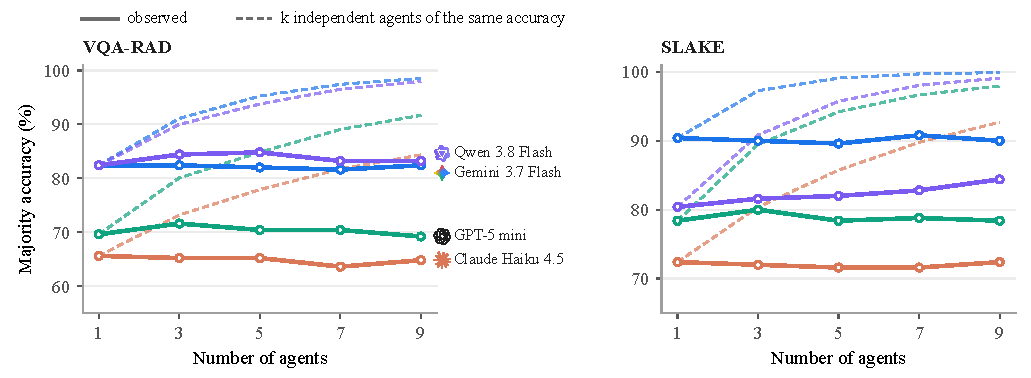
\includegraphics[width=\textwidth]{board_scalingA.pdf}\end{figure}
\begin{figure}[H]\centering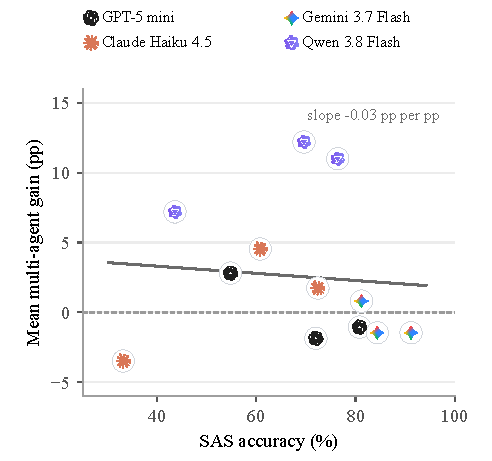
\includegraphics[width=\colw]{board_capabilityA.pdf}\end{figure}
\clearpage
\subsection*{B \quad Pastel soft: NMI pastel family, tinted panels, white grid, no spines}
\begin{figure}[H]\centering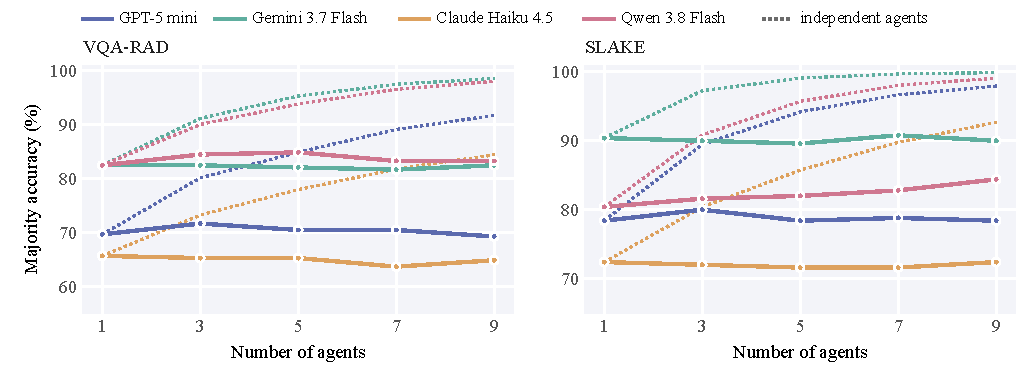
\includegraphics[width=\textwidth]{board_scalingB.pdf}\end{figure}
\begin{figure}[H]\centering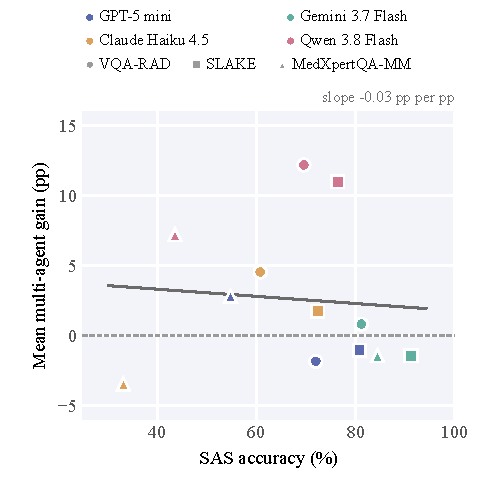
\includegraphics[width=\colw]{board_capabilityB.pdf}\end{figure}
\clearpage
\subsection*{C \quad Editorial: systems in grey, one accent for the key comparison, statements at the line ends}
\begin{figure}[H]\centering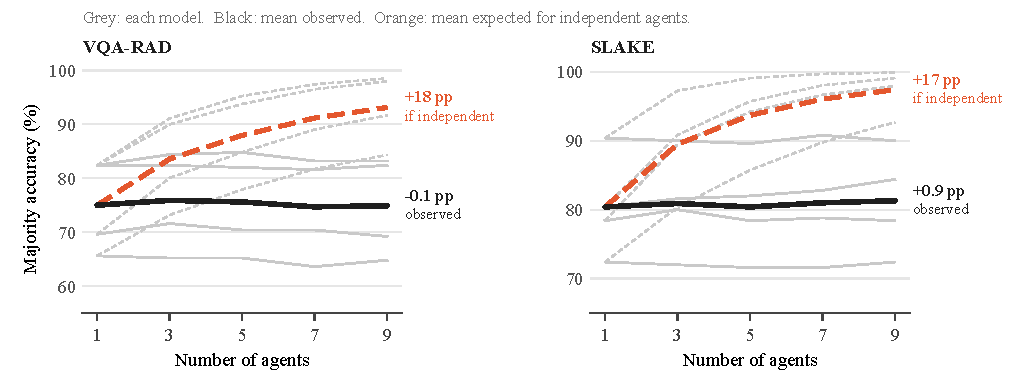
\includegraphics[width=\textwidth]{board_scalingC.pdf}\end{figure}
\begin{figure}[H]\centering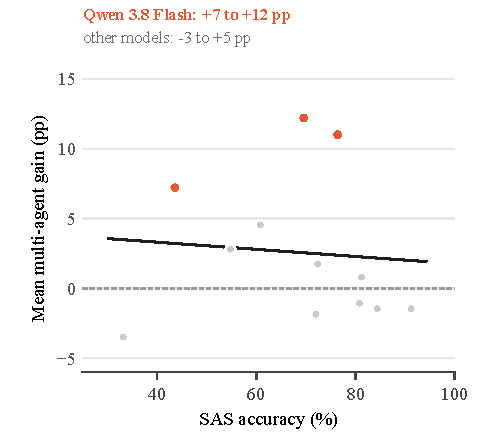
\includegraphics[width=\colw]{board_capabilityC.pdf}\end{figure}
\end{document}
